\documentclass{weekly}
\begin{document}
\maketitlew{Аналитическая механика}{1}{2}{5}

\paragraph{3.6.} Плоская фигура движется в~своей плоскости.
Найти положение точки~$A$, если известны скорость этой точки~$\vec v_A$,
скорость некоторой другой точки~$\vec v_0$ и~угловая скорость
фигуры~$\vec\omega$. Использовать полученный результат для~определения
положения мгновенного центра скоростей~$P$.

$\blacktriangleright$ По~теореме о~распределении скоростей
в~твёрдом теле
\begin{equation}\label{3.6:vA}
    \vec v_A = \vec v_0 + \vec\omega \times \overline{OA}.
\end{equation}
Умножим векторно уравнение~\eqref{3.6:vA} на~$\vec\omega$ слева:
\begin{gather}
    \vec\omega \times \left(\vec v_A - \vec v_0\right) =
            \vec\omega \times \vec\omega \times \overline{OA}
        = \vec\omega \cancelto{0}
            {\left(\vec\omega, \overline{OA}\right)}\quad -
            \overline{OA} \left(\vec\omega, \vec\omega\right)
        = -\omega^2 \cdot \overline{OA}; \\[\parskip]
    \overline{OA} = \frac{\vec\omega \times
            \left(\vec v_0 - \vec v_A\right)}{\omega^2}.
\end{gather}
В~частности, для~мгновенного центра скоростей~$P$ можно записать
$\vec v_P = \vec 0$.\\[-\parskip]

\textbf{Ответ:}\quad $\overline{OA} = \dfrac{\vec\omega \times
\left(\vec v_0 - \vec v_A\right)}{\omega^2}$;\qquad
$\overline{OP} = \dfrac{\vec\omega \times \vec v_0}{\omega^2}$.
\hfill $\blacktriangleleft$


\begin{wrapfigure}[8]{r}{4.5cm}\vspace{-6mm}
    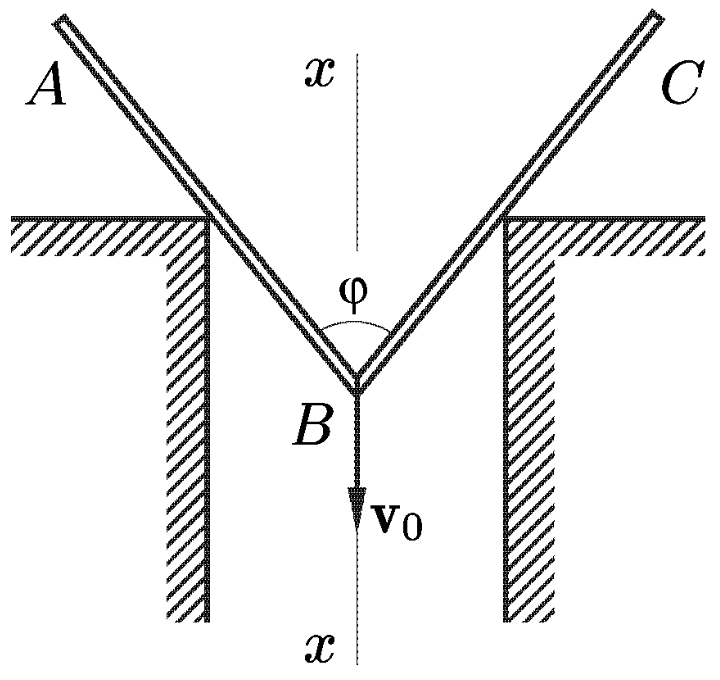
\includegraphics[width=4.5cm]{3-12}
\end{wrapfigure}
\paragraph{3.12.} Стержни~$AB$ и~$BC$ шарнирно соединены в~точке~$B$
и~опираются на~два прямых угла, как~показано на~рисунке.
Точка~$B$ движется по~прямой~$xx$, равноудалённой от~вертикальных сторон
углов. Во~время движения стержни касаются вершин прямых углов.
Доказать, что~скорость точки касания каждого стержня вершин прямого угла
направлена вдоль стержня. Найти также скорости этой точки в~зависимости
от~угла~$\angle ABC = \varphi$, если~скорость точки~$B$ равна~$v_0$.

$\blacktriangleright$ Введём неподвижную систему координат~$T\xi\eta$
в~точке~$T$ касания стержнем угла в~данный момент времени;
ось~$\xi$ направим вдоль стержня,
ось~$\eta$~--- перпендикулярно названному направлению.
Точка~$T$ имеет скорость
\begin{equation}\label{3.12:vT}
    \vec v_O = v_\xi \mathbf{e_\xi} + v_\eta \mathbf{e_\eta}.
\end{equation}
Требуется показать, что~$v_\eta = 0$. В~самом деле, рассмотрим
точку~$A$ стержня с~координатами~$(\delta \xi; 0)$,
которая станет точкой касания через промежуток времени~$\delta t$.
С~одной стороны, понятно, что
\begin{equation}\label{3.12:vA}
    \vec v_A = \frac{\delta \xi}{\delta t} \,\mathbf{e_\xi};
\end{equation}
с~другой стороны, по~теореме Эйлера
\begin{equation}\label{3.12:Euler}
    \vec v_A = \vec v_T + \vec\omega \times \overline{TA}.
\end{equation}

Используя~\eqref{3.12:vT} и~\eqref{3.12:vA}, запишем~\eqref{3.12:Euler}
в~<<проекциях>>:
\begin{equation}
    \frac{\delta\xi}{\delta t} \,\mathbf{e_\xi}
        = v_\xi \mathbf{e_\xi} + v_\eta \mathbf{e_\eta} -
            \omega\,\delta\xi \cdot
            \left(\mathbf{[e_\xi \times e_\eta] \times
                \mathbf{e_\xi}}\right)
        = v_\xi \mathbf{e_\xi} + v_\eta \mathbf{e_\eta} +
            \omega\,\delta\xi \,\mathbf{e_\eta}.
\end{equation}
Таким образом, $v_\eta = \omega \,\delta\xi \to 0$,
что~и требовалось доказать. \qed

Проекции скоростей точек стержня
на~ось~$\xi$ равны между собой (это, между прочим, побочный результат
приведённого выше доказательства). В~силу симметрии системы
нетрудно записать искомый результат.

\textbf{Ответ:}\quad $v_T = v_B \cos\dfrac{\varphi}{2}$.
\hfill $\blacktriangleleft$


\paragraph{3.15.} Плоская фигура движется в~своей плоскости,
причём~её угловая скорость равна~$\omega$. Найти радиус кривизны
траектории точки~$A$ фигуры, если известны ускорение
этой точки~$\vec w_A$ и~положение мгновенного центра скоростей~$P$.

$\blacktriangleright$ Радиус кривизны траектории точки выражается
через её нормальное ускорение. Дальнейший ход решения
состоит в~следующей выкладке:
\begin{equation}
    \rho = \frac{v^2}{w_n}
        = \frac{\abs{\vec\omega \times \overline{PA}}^2}
            {\sqrt{\vec w_A^2 - \left(\vec w_A, \vec\tau\right)^2}}
        = \frac{\abs{\vec\omega \times \overline{PA}}^3}
            {\abs{\vec w_A \times \vec v}}
        = \frac{\abs{\vec\omega \times \overline{PA}}^3}
            {\abs{\vec w_A \times \vec\omega \times \overline{PA}}}
        = \frac{\omega^2 \abs{\overline{PA}}^3}
            {\abs{\left(\vec w_A, \overline{PA}\right)}}.
\end{equation}

\textbf{Ответ:}\quad $\rho = \dfrac{\omega^2 \abs{\overline{PA}}^3}
{\abs{\left(\vec w_A, \overline{PA}\right)}}$.
\hfill $\blacktriangleleft$


\begin{wrapfigure}[7]{r}{6cm}\vspace{-6mm}
    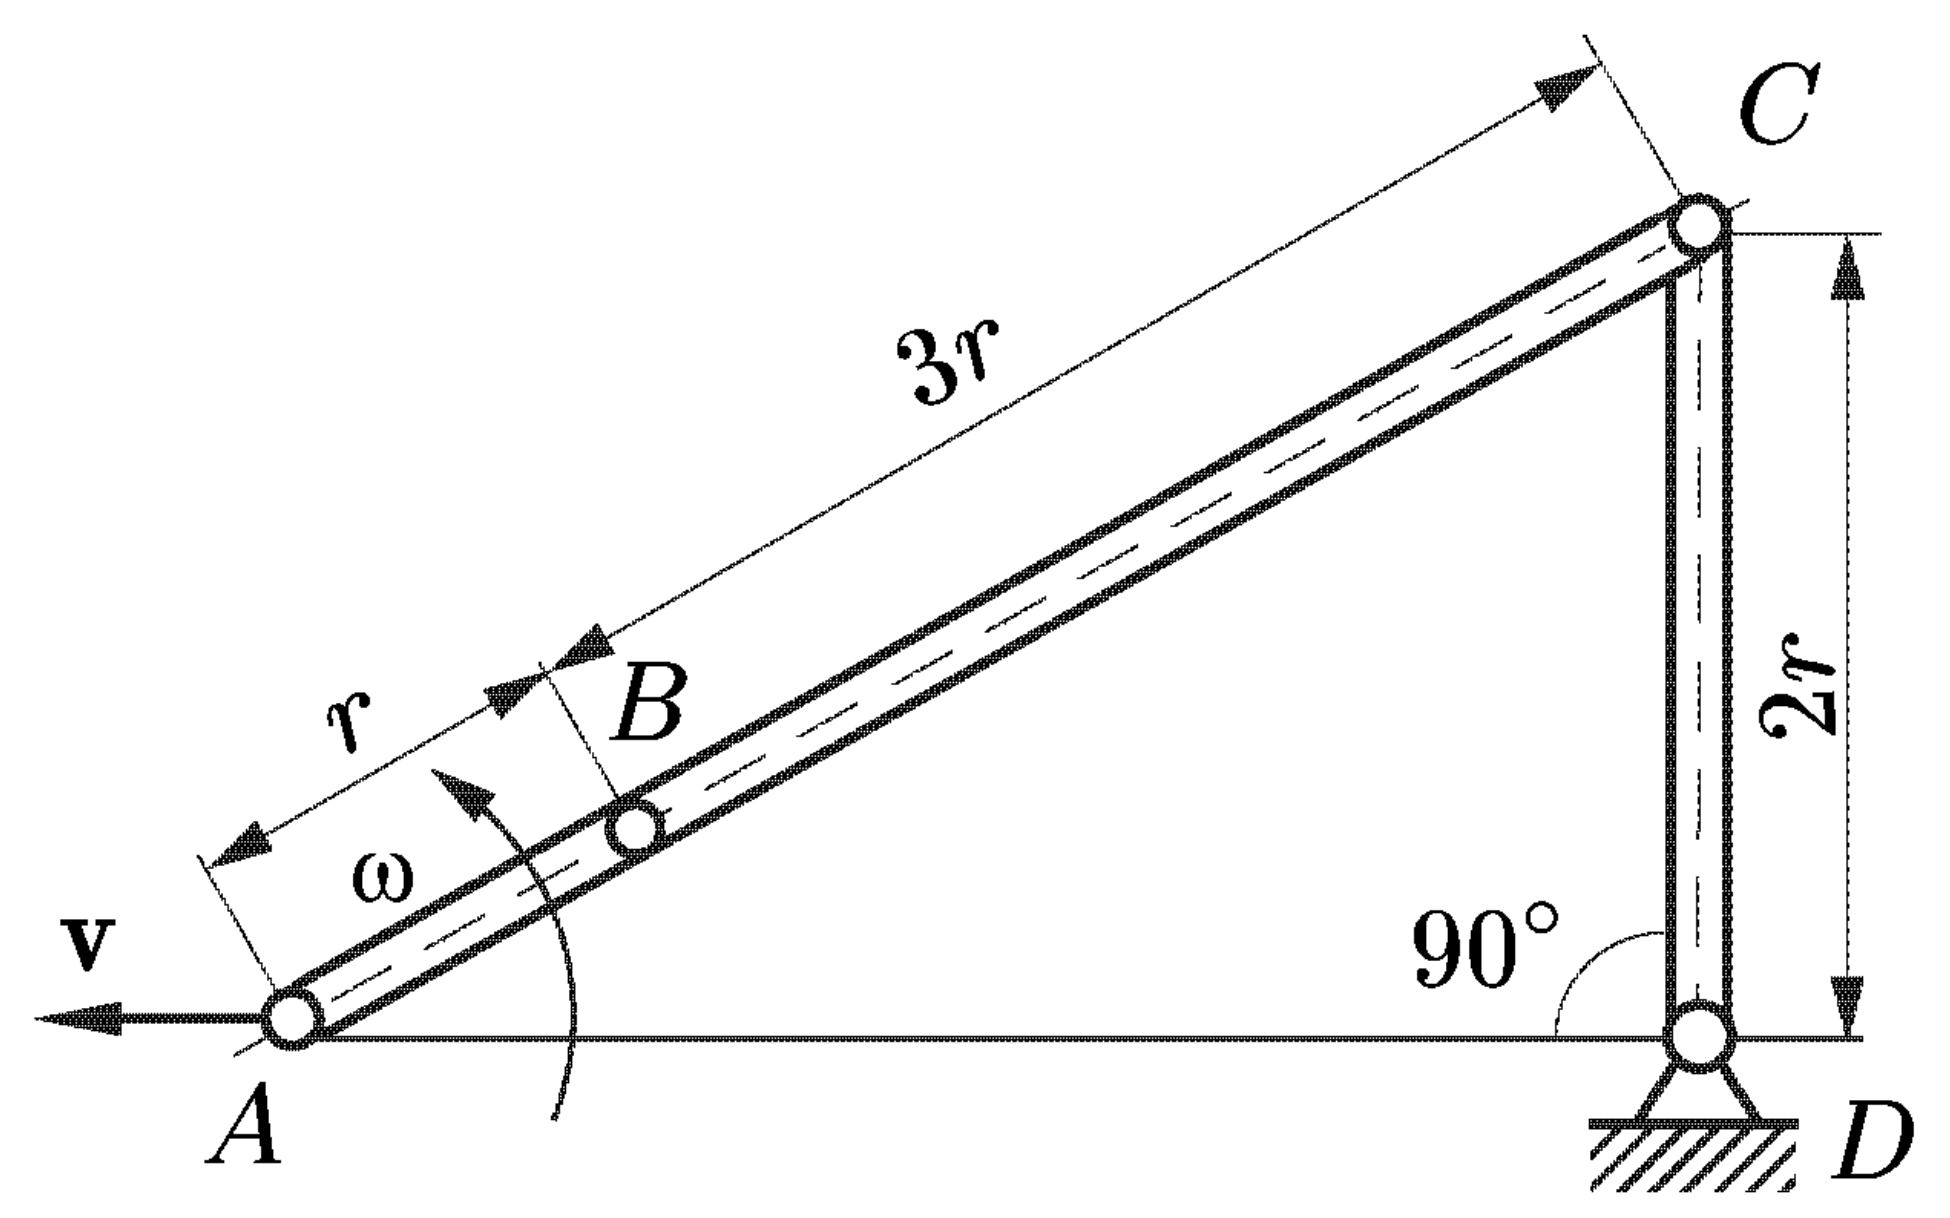
\includegraphics[width=6cm]{3-24}
\end{wrapfigure}
\paragraph{3.24.} Стержни~$AB$, $BC$ и~$CD$ соединены шарнирами,
причём стержень~$CD$ может поворачиваться вокруг неподвижной точки~$D$,
а~стержень~$AB$ вращается с~постоянной угловой скоростью~$\vec\omega$
вокруг точки~$A$, движущейся по~прямой~$AD$ с~постоянной
скоростью~$\vec v$. Найти скорость и~ускорение точки~$C$ в~момент,
когда $\angle ABC = 180^\circ$, а~$\angle ADC = 90^\circ$.

$\blacktriangleright$ Введём координатные оси на~плоскости следующим
образом: ось~$x$ направим вдоль $DA$, ось~$y$~--- вдоль~$DC$.
Дополним координатную систему осью~$z$ до~правой тройки:
$\mathbf{e_z} = \mathbf{e_x} \times \mathbf{e_y}$.

Введём для~краткости обозначение~$\psi \equiv \angle DAC = 30^\circ$
и~запишем скорость точки~$C$ двумя способами:
\begin{align}
    \vec v_C &= \vec\omega_{DC} \times \overline{DC}
        = \cvec{0}{0}{\omega_{DC}} \times \cvec{0}{2r}{0}
        = \cvec{-2r\omega_1}{0}{0}; \\[2ex]
\begin{split}
    \vec v_C &= \vec v_B + \vec\omega_{BC} \times \overline{BC}
        = \vec v_A + \vec\omega_{AB} \times \overline{AB} +
            \vec\omega_{BC} \times \overline{BC} =\\
        &= \cvec{v}{0}{0} + r \cvec{0}{0}{\omega} \times
            \cvec{-\cos\psi}{\sin\psi}{0} +
            3r \cvec{0}{0}{\omega_2} \times
            \cvec{-\cos\psi}{\sin\psi}{0}
        = \cvec{v - (\omega - 3\omega_2) r\sin\psi}
            {-(\omega - 3\omega_2) r\cos\psi}{0}. \label{3.24:vC2}
\end{split}
\end{align}

Приравнивая компоненты вектора~$\vec v_C$, приходим к~системе уравнений
\begin{gather}
    \begin{cases}
        -2r\omega_1 = v - (\omega - 3\omega_2) r\sin\psi; \\
        0 = -(\omega - 3\omega_2) r\cos\psi.
    \end{cases}
    \then
    \begin{cases}
        \omega_1 = -v/{2r};\\
        \omega_2 = \omega/3.
    \end{cases}
\end{gather}
Пристальный взгляд на~\eqref{3.24:vC2} позволяет установить,
что~$\vec v_C = \vec v$.

Теперь займёмся ускорениями:
\begin{align}
\begin{split}
    \vec w_C &= \vec\varepsilon_{DC} \times \overline{DC} +
            \vec\omega_{DC} \times \vec\omega_{DC} \times \overline{DC}
        = \vec\varepsilon_{DC} \times \overline{DC} -
            \omega_1^2 \cdot \overline{DC} = \\
        &= \cvec{0}{0}{\varepsilon_1} \times \cvec{0}{2r}{0} +
            \cvec{0}{-\omega_1^2 \cdot 2r}{0}
        = \cvec{-2\varepsilon_1 r}{-v^2/(2r)}{0};
\end{split} \\[1ex]
\begin{split}
    \vec w_C &= \vec w_B + \vec\varepsilon_{BC} \times \overline{BC} -
            \omega_2^2 \cdot \overline{BC}
        = -\omega^2 \cdot \overline{AB} -
            \omega_2^2 \cdot \overline{BC} +
            \vec\varepsilon_{BC} \times \overline{BC} = \\
        &= \cvec{\left(\omega^2 + 3\omega_2^2\right) r\cos\psi}
            {-\left(\omega^2 + 3\omega_2^2\right) r\sin\psi}{0} +
            3r \cvec{0}{0}{\varepsilon_2} \times
            \cvec{-\cos\psi}{\sin\psi}{0}
        = \cvec{\frac{4}{3} \omega^2 \cos\psi -
                3\varepsilon_2 \sin\psi}
            {-\frac{4}{3} \omega^2 \sin\psi -
                3\varepsilon_2 \cos\psi}{0} r.
\end{split}
\end{align}
Теперь нетрудно уже вновь перейти к~системе уравнений:
\begin{gather}
    \begin{cases}
        -4\sqrt{3}\varepsilon_1 = 4\omega^2 -
            3\sqrt{3}\varepsilon_2; \\
        v^2/r^2 = \frac{4}{3}\omega^2 +
            3\sqrt{3}\varepsilon_2.
    \end{cases}
    \then
    -4\sqrt{3}\varepsilon_1 + \frac{v^2}{r^2} = \frac{16}{3}\omega^2.
\end{gather}\\[-5ex]
\begin{align}
    \vec\omega_C &= \cvec
        {\frac{\sqrt{3}}{6}
        \left( \frac{16}{3}\omega^2 r - v^2/r \right)}
        {-\frac{1}{2} v^2/r}
        {0}; \\
    \omega_C &= \sqrt{\frac{64}{27} \omega^4 r^2 +
            \frac{1}{3} \frac{v^4}{r^2} - \frac{8}{9} \omega^2 v^2}.
\end{align}

\textbf{Ответ:}\quad $\vec v_C = \vec v$;\qquad
$\vec w_C = \cvec
    {\frac{\sqrt{3}}{6}\left( \frac{16}{3}\omega^2 r - v^2/r \right)}
    {-\frac{1}{2} v^2/r}{0}$.
\hfill $\blacktriangleleft$


\begin{wrapfigure}[7]{l}{4.3cm}\vspace{3mm}
    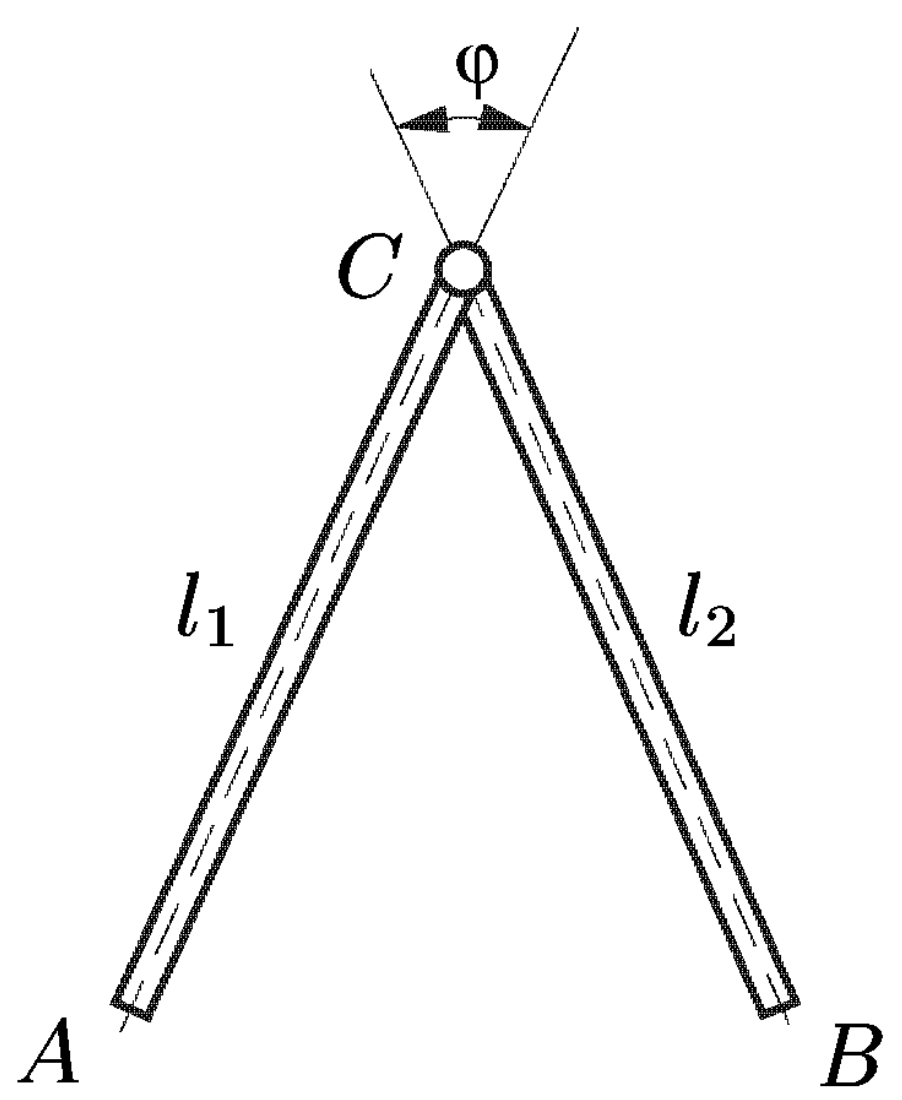
\includegraphics[width=4.3cm]{3-33}
\end{wrapfigure}
\paragraph{3.33.} Стержни~$AC$ и~$BC$ длины~$l_1$ и~$l_2$
соответственно, соединённые в~точке~$C$ шарниром, движутся
в~плоскости. Известны скорости свободных концов стержней~$\vec v_A$
и~$\vec v_B$, а~также их~ускорения~$\vec w_A$ и~$\vec w_B$.
Найти угловые скорости и~угловые ускорения стержней, если
угол между ними в~рассматриваемый момент времени равен~$\varphi$
($0 < \varphi < \pi$).

$\blacktriangleright$ Запишем скорость и~ускорение точки~$C$
двумя способами:
\begin{align}
    \vec v_C &= \vec v_A + \vec\omega_1 \times \overline{AC},
        \label{3.33:vC1}\\
    \vec v_C &= \vec v_B + \vec\omega_2 \times \overline{BC};
        \label{3.33:vC2}\\[1.5ex]
    \vec w_C &= \vec w_A + \vec\varepsilon_1 \times \overline{AC} -
        \omega_1^2 \cdot \overline{AC}, \label{3.33:wC1}\\
    \vec w_C &= \vec w_B + \vec\varepsilon_2 \times \overline{BC} -
        \omega_2^2 \cdot \overline{BC}. \label{3.33:wC2}
\end{align}

Умножим уравнения~\eqref{3.33:vC1} и~\eqref{3.33:vC2} скалярно
на~$\overline{BC}$ и~исключим~$\vec v_C$:
\begin{gather}
    \left(\vec v_A, \overline{BC}\right) +
            \left(\overline{BC}, \vec\omega_1, \overline{AC}\right)
        = \left(\vec v_B, \overline{BC}\right) +
            \cancel{\left(\overline{BC},
            \vec\omega_2, \overline{BC}\right)}, \\
    \left(\vec\omega_1, \overline{BC}, \overline{AC}\right)
        = \left(\vec v_A - \vec v_B, \overline{BC}\right), \\
    \omega_1 = \frac{\left(\vec v_A - \vec v_B\right)\cdot\overline{BC}}
        {l_1 l_2 \sin\varphi}.
\end{gather}
Для~нахождения другой угловой скорости умножим те~же уравнения
скалярно на~$\overline{AC}$:
\begin{gather}
    \left(\vec v_A, \overline{AC}\right) +
            \cancel{\left(\overline{AC},
            \vec\omega_1, \overline{AC}\right)}
        = \left(\vec v_B, \overline{AC}\right) +
            \left(\overline{AC}, \vec\omega_2, \overline{BC}\right), \\
    \left(\vec\omega_1, \overline{AC}, \overline{BC}\right)
        = \left(\vec v_B - \vec v_A, \overline{AC}\right), \\
    \omega_2 = \frac{\left(\vec v_B - \vec v_A\right)\cdot\overline{AC}}
        {l_1 l_2 \sin\varphi}.
\end{gather}

Теперь умножим уравнения~\eqref{3.33:wC1} и~\eqref{3.33:wC2}
скалярно на~$\overline{BC}$ и~исключим~$\vec w_C$:
\begin{gather}
    \left(\vec w_A, \overline{BC}\right) +
            \left(\overline{BC}, \vec\varepsilon_1,
            \overline{AC}\right) -
            \omega_1^2 \cdot \left(\overline{AC}, \overline{BC}\right)
        = \left(\vec w_B, \overline{BC}\right) %+
            %\cancel{\left(\overline{BC}, \vec\varepsilon_2,
            %\overline{BC}\right)}
            - \omega_2^2 \cdot \left(\overline{BC},
            \overline{BC}\right), \\
    \varepsilon_1 = \frac{\left(\vec w_B - \vec w_A\right) \cdot
            \overline{BC} - \omega_2^2 l_2^2 +
            \omega_1^2 l_1 l_2 \cos\varphi}{l_1 l_2 \sin\varphi}.
\end{gather}
Аналогично для~$\varepsilon_2$:
\begin{gather}
    \left(\vec w_A, \overline{AC}\right) %+
            %\cancel{\left(\overline{AC}, \vec\varepsilon_1,
            %\overline{AC}\right)}
            - \omega_1^2 \cdot \left(\overline{AC}, \overline{AC}\right)
        = \left(\vec w_B, \overline{AC}\right) +
            \left(\overline{AC}, \vec\varepsilon_2,
            \overline{BC}\right) -
            \omega_2^2 \cdot \left(\overline{AC},
            \overline{BC}\right), \\
    \varepsilon_2 = \frac{\left(\vec w_B - \vec w_A\right) \cdot
            \overline{AC} + \omega_1^2 l_1^2 -
            \omega_2^2 l_1 l_2 \cos\varphi}{l_1 l_2 \sin\varphi}.
\end{gather}

\textsl{Примечание.} Направления искомых векторов
без ограничения общности можно установить,
используя частный случай, например, ситуацию, когда
точка $C$ является мгновенным центром скоростей стержней.
Безусловно, эти векторы ортогональны плоскости рисунка.

\textbf{Ответ:}\quad
$\omega_1 = \dfrac{\left(\vec v_A - \vec v_B\right)\cdot\overline{BC}}
    {l_1 l_2 \sin\varphi}$;\qquad
$\omega_2 = \dfrac{\left(\vec v_B - \vec v_A\right)\cdot\overline{AC}}
    {l_1 l_2 \sin\varphi}$;\\[1.5ex]
$\varepsilon_1 = \dfrac{\left(\vec w_B - \vec w_A\right) \cdot
    \overline{BC} - \omega_2^2 l_2^2 +
    \omega_1^2 l_1 l_2 \cos\varphi}{l_1 l_2 \sin\varphi}$;\qquad
$\varepsilon_2 = \dfrac{\left(\vec w_B - \vec w_A\right) \cdot
    \overline{AC} + \omega_1^2 l_1^2 -
    \omega_2^2 l_1 l_2 \cos\varphi}{l_1 l_2 \sin\varphi}$.
\hfill $\blacktriangleleft$

\end{document}
